\section{Klient webowy - pilot uruchomiony na urządzeniu mobilnym}

Kluczowym z punktu widzenia systemu jest poprawnie działający, uniwersalny klient webowy w postaci strony internetowej wyświetlanej w przeglądarce na urządzeniu mobilnym klienta końcowego. Biorąc pod uwagę różnorodność rozdzielczości ekranów, gęstości pikseli (ang. \emph{pixel density}), szybkości wykorzystywanych łącz, wsparcia przeglądarek internetowych na urządzeniach mobilnych dla dyrektyw CSS 3\footnote{CSS (ang. \emph{Cascading Style Sheets}) kaskadowe arkusze stylów, opisujące sposób wyświetlania elementów strony internetowej)}, SVG\footnote{SVG (ang. \emph{Scalable Vector Graphics}) format grafiki wektorowej} rozpoznano szereg problemów oraz zaproponowano rozwiązania.

\subsection{Wykrywanie gestów telefonu komórkowego}

Pojawienie się na rynku urządzeń dotykowych postawiły przed twórcami interfejsów nowe wyzwania, a projektantom mobilnych przeglądarek internetowych wyzwanie obsługi gestów wykonywanych palcami na ekranie i ich interpretacje na istniejące już, dobrze zakorzenione standardy obsługi zdarzeń myszy.

Przeglądarki internetowe uruchamiane na urządzeniach mobilnych, które przewidują dotykowy sposób komunikacji z interfejsem aplikacji internetowej zazwyczaj odwzorowują dotyk jako zdarzenia myszy (ang. \emph{mouse events}), aby umożliwić interakcję z uruchomioną na ekranie aplikacją. Niestety interpretacja dotyku jako zdarzeń myszy ma pewne ograniczenia użyteczności związane z fizycznym dostępem do treści. Co więcej, w przeglądarce internetowej nie ma możliwości obsługi wielu kursorów jako dotyku kilku palców jednocześnie, ze względu na ograniczenia interfejsu zdarzeń myszy, niezależnie od możliwości urządzenia. Oba te ograniczenia, na poziomie systemowym oraz ze względu na wsteczną zgodność standardów rodzą problemy z obsługą dotyku jako zdarzeń.

\subsubsection{W3C Touch Events specification}

Specyfikacja zdarzeń dotyku (\emph{Touch Events specification}\cite{touch-events-w3c}) opracowana przez W3C\footnote{W3C - World Wide Web Consortium} rozwiązuje powyższe problemy definiując interfejsy umożliwiające aplikacjom bezpośrednią obsługę zdarzeń gestów, z możliwością interpretacji wielu dotyków jednocześnie dla urządzeń zdolnych do ich obsługi. Jej pierwsza wersja (\emph{Proposed Recommendation}) powstała już 5 maja 2011, aż po pięciu poprawkach (przechodząc przez statusy \emph{Working Draft} oraz \emph{Candidate Recommendation}) uzyskała status \emph{W3C Recommendation}.

Definiuje ona interfejs punktu dotyku \emph{Touch} jako obiekt niezmienny (ang. \emph{immutable object}\footnote{Immutable object - Obiekt niezmienny raz utworzony, nie może zmieniać swojego stanu}):

\lstset{language=Octave}
\begin{lstlisting}
interface Touch {
    readonly    attribute long        identifier;
    readonly    attribute EventTarget target;
    readonly    attribute long        screenX;
    readonly    attribute long        screenY;
    readonly    attribute long        clientX;
    readonly    attribute long        clientY;
    readonly    attribute long        pageX;
    readonly    attribute long        pageY;
};
\end{lstlisting}

\begin{description}
  \item[identifier] \hfill \\
  Unikatowy identyfikator punktu dotyku względem pozostałych identyfikatorów już aktywnych\footnote{Można wyobrazić sobie sytuację, gdy nowy punkt dotyku pojawia się, gdy użytkownik dotykał powierzchnię w innych miejscach} punktów dotyku. Każdy punkt dotyku otrzymuje identyfikator w momencie jego zarejestrowania.
  \item[target] \hfill \\
  Obiekt na powierzchni który został wskazany przez punkt dotyku w momencie jego zarejestrowania. Nawet, jeżeli punkt dotyku się przesuwa wskazując inne obiekty, target nie ulega zmianie\footnote{Można wykorzystać ten fakt do zmiany położenia zgodnie ze zmianą pozycji punktu dotyku, np. do przesuwania obiektów}.
  \item[screenX, screenY] \hfill \\
  Współrzędne punktu dotyku względem punktu zerowego ekranu.
  \item[clientX, clientY] \hfill \\
  Współrzędne punktu dotyku względem punktu zerowego powierzchni rzutni na której wyświetlana jest strona internetowa, z wyłączeniem przesunięcia punktu widoczności.
  \item[pageX, pageY] \hfill \\
  Współrzędne punktu dotyku względem punktu zerowego powierzchni rzutni na której wyświetlana jest strona internetowa, z uwzględnieniem przesunięcia punktu widoczności (suma przesunięcia oraz pozycji punktu dotyku na widocznej części rzutni).
\end{description}

Ponadto do obsługi wielu punktów dotyku pojawiających się równolegle zdefiniowano interfejs \lstinline{TouchList} zawierający listę punktów dotyku:

\lstset{language=Octave}
\begin{lstlisting}
interface TouchList {
    readonly    attribute unsigned long length;
    getter Touch? item (unsigned long index);
};
\end{lstlisting}

Aby reagować na zdefiniowane zdarzenia, należy zarejestrować procedurę obsługi zdarzenia. Dostępne są następujące zdarzenia:

\begin{description}
  \item[touchstart] \hfill \\
  Zdarzenie jest wyzwalane, gdy wystąpi pojawienie się nowego punktu dotyku. Jego domyślna implementacja nie jest określona.
  \item[touchend] \hfill \\
  Zdarzenie jest wyzwalane, gdy wystąpi zaniknięcie punktu dotyku. Jego domyślna implementacja zakłada, że wyzwalane jest zdarzenie \lstinline{mousemove}, jeżeli punkt dotyku się kiedykolwiek przemieścił lub wyzwolenie zdarzeń \lstinline{mousedown}, \lstinline{mouseup}, \lstinline{click}, gdy punkt nie zmienił swojego położenia\footnote{Imitacja kliknięcia myszą na urządzeniach dotykowych}.
  \item[touchmove] \hfill \\
  Zdarzenie jest wyzwalane, gdy nastąpi zmiana położenia punktu dotyku.
  \item[touchcancel] \hfill \\
  Zdarzenie jest wyzwalane, gdy punkt dotyku opuszcza dostępną rzutnię lub gdy występuje błąd implementacji. Niezdefiniowane zachowanie.
\end{description}

\subsubsection{Respektowanie standardu Touch Events przez producentów przeglądarek}
\label{subsec:w3c-touch-events-implementations}

Pojawienie się propozycji standardu nie gwarantuje, że producenci popularnych przeglądarek internetowych zaimplementują daną funkcjonalność wg podanej specyfikacji, bądź czy obsługa w ogóle występuje. W chwili obecnej biorąc pod uwagę przeglądarki internetowe dla urządzeń mobilnych, standard jest wspierany przez\cite{caniuse-touch-events}:

\begin{enumerate}
  \item \textbf{iOS Safari}\cite{browser-ios-safari} \footnote{\cite{browser-ios-safari} Rozdział \em{Handling events}, \url{https://developer.apple.com/library/ios/documentation/AppleApplications/Reference/SafariWebContent/HandlingEvents/HandlingEvents.html}}, natywna przeglądarka systemu iOS firmy Apple;
  \item \textbf{Android Browser}, natywna przeglądarka systemu Android;
  \item \textbf{Blackberry Browser},
  \item \textbf{Firefox} - określa własny, bardzo podobny standard, dzięki któremu można osiągnąć te same efekty\cite{browser-firefox} \footnote{\cite{browser-firefox} Rozdział \em{Touch events}, \url{https://developer.mozilla.org/en-US/docs/Web/Guide/Events/Touch_events}}.
\end{enumerate}

Przeglądarki nie wspierające standardu:

\begin{enumerate}
  \item \textbf{Opera Mini},
  \item \textbf{IE Mobile}, własny standard, niekompatybilny\cite{browser-ie} \footnote{\cite{browser-ie} Rozdział \em{Pointer and gesture events}, \url{http://msdn.microsoft.com/en-us/library/ie/hh673557(v=vs.85).aspx}}.
\end{enumerate}

\subsubsection{Użycie biblioteki jQuery Mobile}

Brak respektowania standardów stwarza problemy związane z obsługą gestów na urządzeniach mobilnych. Aby zapewnić poprawne funkcjonowanie należy śledzić zmiany wprowadzane w implementacjach przeglądarek przez producentów oraz ewentualne zmiany w standardach. W projekcie wykorzystana została biblioteka \emph{jQuery Mobile} posiadająca dużą społeczność\footnote{Ponad 10 tyś poprawek, 36 wersji, 204 osób wnoszących wkład w rozwój biblioteki [Stan na 22 grudnia 2013]}. Wśród wpieranych przeglądarek znajdują się wymienione jako niewspierające standardu z podsekcji ~\ref{subsec:w3c-touch-events-implementations}.

Biblioteka wykorzystywana w zakresie poruszania punktów dotyków definiuje \emph{wirtualną mysz} (oznaczoną \lstinline{vmouse}) jako abstrakcję na standardową mysz lub dotyk na urządzeniu mobilnym. Zdarzenia obsługujące wirtualną mysz będą wyzwalane dla myszy komputerowej oraz dla panelu dotykowego.

Zdarzenie \lstinline{vmousemove} symuluje zdarzenia \lstinline{onmousemove} oraz \lstinline{touchmove}. Przykład użycia:

\lstset{language=JavaScript}
\begin{lstlisting}
$(document).on('vmousemove', function(e) {
	// Zapobieganie dalszej propagacji zdarzenia
	// po przechwyceniu, strona nie bedzie przewijana.
	e.preventDefault();
	
	// Pobieranie pozycji kursora z obiektu zdarzenia.
	var x = e.pageX
	var y = e.pageY
	
	console.log(x, y) // wypisz dane na konsoli
})
\end{lstlisting}

\subsubsection{Reprezentacja kursora na płaszczyźnie}

Kursor jest reprezentowany za pomocą punktu \(C(x_{c}, y_{c})\) o nieujemnych, całkowitych współrzędnych \emph{cursor coordinate} oznaczających jego pozycję od punktu \(P(0, 0)\) umieszczonego w lewym, górnym rogu ekranu, a wektor jest skierowany ku punktowi w prawym, dolnym rogu ekranu.

\begin{figure}[h!]
  \caption{Sposób wyznaczania pozycji kursora myszy.}
  \centering
    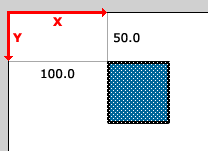
\includegraphics{wyznaczanie-pozycji-kursora}
\end{figure}

Uwzględniając różne proporcje \(p = \frac{szerokosc}{wysokosc}\) ekranu na którym pojawia się zdalnie sterowany kursor oraz proporcje powierzchni ekranu urządzenia mobilnego, w implementacji pilota użyta została reprezentacja procentowa punktu na ekranie.

Pozycja kursora reprezentowana jest przez punkt \(P(x, y)\) na dwuwymiarowej płaszczyźnie w zakresie \( x\in \langle0, 1\rangle \), gdzie \(x = \frac{x_{c}}{w_{x}}\), \(y = \frac{x_{c}}{w_{y}}\), a \(w_{x}\) oraz \(w_{y}\) oznaczają kolejno szerokość i wysokość ekranu.

Wyznaczanie pozycji uwzględnia również zmianę orientacji (poziomej lub pionowe), szerokości i wysokości rzutni okna przeglądarki wyświetlanej na urządzeniu mobilnym.

\lstset{language=JavaScript}
\begin{lstlisting}
this.run = function() {
	
	var this = that
	this.windowX = 0
	this.windowY = 0
	
	$(document).on('vmousemove', function(e) {
		e.preventDefault(); // prevent scroll
		
		var x = e.pageX / that.windowX
		var y = e.pageY / that.windowY
		
		console.log(x, y) // wypisz punkty
	})
	
	var indicateWindowSize = function() {
		that.windowX = $(window).width()
		that.windowY = $(window).height()
	}
	
	// register window size changes listeners
	$(window).on('resize orientationchange', function() {
		indicateWindowSize()
	})
	indicateWindowSize()
}
\end{lstlisting}

\subsection{Pamięć podręczna Web Storage}

Klient webowy uruchomiony na urządzeniu mobilnym zawiera pliki z kodem JavaScript, które są pobierane do przeglądarki internetowej celem ich interpretacji i późniejszego wykonania. Ze względu na specyfikę sieci 3G: mniejsza przepustowość (ang. \emph{bandwidth}), koszt transferu (ponoszony przez użytkownika końcowego), większe opóźnienia (ang. \emph{latency}) niezbędnym jest zapamiętywanie lokalnie pobranych plików, celem ich ponownego otwarcia z lokalnej przestrzeni dyskowej urządzenia, bez konieczności dostępu do nich przez sieć.

Przeglądarki internetowe na urządzeniach mobilnych wspierają pamięć tymczasową \emph{cache} protokołu HTTP opisaną w dokumencie RFC-2616 \emph{Hypertext Transfer Protocol - HTTP/1.1}\cite{http-rfc} \footnote{Rozdział 13, \emph{Caching in HTTP}}. Można by było zadać pytanie, czy pamięć jest zachowywana po zamknięciu przeglądarki na urządzeniu mobilnym jako aplikacji, przy blokowaniu i wyłączaniu telefonu. Wykonane testy dowodzą, że przeglądarki internetowe na urządzeniach mobilnych wykazują poprawne zachowanie\cite{http-cache-mobile-benchmark}.

Można by było zaprzestać na serwowaniu plików JavaScript z nagłówkiem \lstinline{Cache-Control} oraz \lstinline{Expires} na bardzo odległy czas, przykładowo:

\lstset{language=Octave}
\begin{lstlisting}
Cache-Control: max-age=315360000, must-revalidate
Expires: Mon, 30 Oct 2023 14:19:41 GMT
\end{lstlisting}

Zaproponowany standard W3C \emph{Web Storage}\cite{webstorage}\footnote{W3C Recommendation, {\em Web Storage}, \url{http://www.w3.org/TR/webstorage/}}, który również zapewnia przechowywanie danych lokalnie, dał początek testom związanych z szybkością ładowania plików z obu pamięci podręcznych. Local Storage to pamięć asocjacyjna klucz-wartość (ang. \emph{key-value storage}), gdzie zarówno klucz, jak i wartość są ciągiem znaków. Wartości JavaScript nie będące ciągiem znaków są na niego rzutowane.

Co prawda, w swoim zamierzeniu Web Storage nie miał na celu przechowywanie plików wchodzących w skład strony internetowej, ale posiada interfejs, który umożliwia wykorzystanie go właśnie w ten sposób. Wykonane testy wykazały, że ładowanie danych z Web Storage (dokładniej \emph{Local Storage}) jest nawet do 5 razy szybsze, niż w przypadku ładowania danych z pamięci podręcznej przeglądarki (\emph{Native cache})\cite{http-cache-mobile-benchmark}\footnote{Testy dotyczące przeglądarek internetowych na urządzeniach mobilnych opublikowanych 13 maja 2013 przez Petera McLachlana}:

\begin{figure}[h!]
  \caption[Porównanie czasu ładowania danych z cache przeglądarki oraz Web Storage]{Czerwoną kreską oznaczono średnią.}
  \centering
    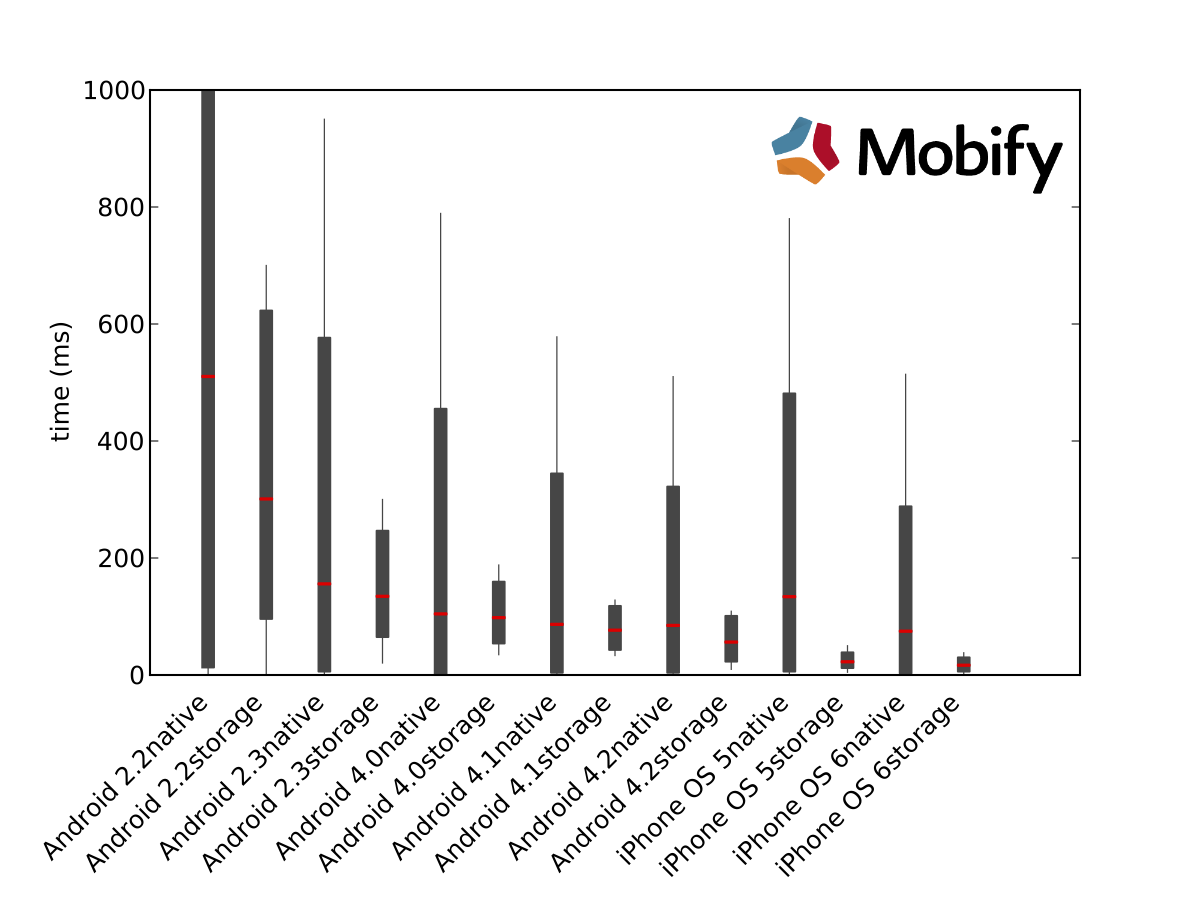
\includegraphics[width=\textwidth]{localstorage-benchmark}
\end{figure}

\begin{center}
    \begin{tabular}{ | l | p{2.5cm} | p{2.5cm} | p{2.5cm} | p{2.5cm} |}
    \hline
	Smartphone OS & localStorage \newline śr. (ms) & native browser \newline śr. (ms) & localstorage \newline odch. st. & native browser \newline odch. st. \\ \hline
	Android 2.2 & 299.94 & 509.32 & 164.76 & 537.95 \\ \hline
	Android 2.3 & 133.50 & 154.76 & 57.65 & 215.13 \\ \hline
	Android 4.0 & 97.05 & 103.44 & 31.80 & 179.36 \\ \hline
	Android 4.1 & 75.60 & 85.57 & 21.60 & 132.03 \\ \hline
	Android 4.2 & 55.28 & 83.76 & 23.28 & 121.51 \\ \hline
	iPhone iOS5 & 21.61 & 132.90 & 8.64 & 177.69 \\ \hline
	iPhone iOS6 & 15.71 & 73.86 & 7.27 & 109.32 \\ \hline
    \hline
    \end{tabular}
\end{center}

W przypadku Local Storage zarówno średni czas ładowania, jak i wariancja i odchylenie standardowe jest znacznie mniejsze.

Dokument standardu W3C\cite{webstorage} definiuje sposób dostępu do danych z pamięci lokalnej przeglądarki. Propozycja wynikła z faktu, iż dane zachowane lokalnie w przeglądarce internetowej przed jego pojawieniem się, implementowane za pomocą mechanizmu ciasteczek (ang. \emph{Cookies}) brały udział w transmisji w protokole HTTP jako dane nagłówkowe wychodzące od strony klienta do serwera, co nie było pożądane ze względu na dodatkowy narzut transmisji. Ponadto serwer jest świadom istnienia danych lokalnych i jest w stanie je odebrać (nagłówek HTTP \lstinline{Cookie: } podczas wysyłania żądania do serwera) oraz, co gorsza modyfikować (nagłówek HTTP \lstinline{Set-Cookie: } podczas wysyłania odpowiedzi od serwera).

Przykładowe żądanie HTTP z ciasteczkiem:
\lstset{language=Octave}
\begin{lstlisting}
GET / HTTP/1.1
Host: www.example.org
Cookie: name=value; name2=value2
Accept: */*
\end{lstlisting}

Przykładowa odpowiedź HTTP z modyfikacją ciasteczka:
\lstset{language=Octave}
\begin{lstlisting}
HTTP/1.0 200 OK
Content-type: text/html
Set-Cookie: name=value
Set-Cookie: name2=MODIFIED_VALIE; Expires=Wed, 09 Jun 2021 10:18:14 GMT

(content of page)
\end{lstlisting}

Standard definiuje pamięć jako interfejs \emph{Storage}, na którym można dokonywać operacji odczytu, zapisu, usunięcia.

\lstset{language=Octave}
\begin{lstlisting}
interface Storage {
  readonly attribute unsigned long length;
  DOMString? key(unsigned long index);
  getter DOMString? getItem(DOMString key);
  setter creator void setItem(DOMString key, DOMString value);
  deleter void removeItem(DOMString key);
  void clear();
};
\end{lstlisting}

Istnieją dwa rodzaje pamięci:

\begin{description}
  \item[Local Storage] \hfill \\
  Przypisany dla danego źródła \emph{Origin}\footnote{Origin to zestaw wartości w postaci: \emph{protocol://domain:port}, gdzie \emph{protocol} to skrótowa nazwa protokołu (np http, https), \emph{domain} to nazwa hosta oraz \emph{port} to numer portu, pod którym jest uruchomiona dana usługa} a trybucie \emph{document} pamięć typu \emph{Storage}. Oznacza to, że każda strona internetowa otwarta w przeglądarce posiada swoją niezależną pamięć podręczną, niedostępną dla stron internetowych uruchomionych z innego adresu (protokół, nazwa hosta, numer portu). \emph{Same Origin Policy} zapewnia, że jedna pamięć może być dzielona tylko i wyłącznie między dokumentami otwartymi przez przeglądarkę dla tej samej nazwy hosta, uruchomiona na wybranym, określonym porcie oraz przekazywana jednym określonym protokołem (np. http, czy https). Dla każdej różnej kombinacji tworzona jest oddzielna pamięć, a dokumenty nie mają dostępu do swoich pamięci na wzajem. Pamięć \emph{Local Storage} ma nieograniczony czas życia, nie ulega zdezaktualizowaniu, dopóki nie zabraknie limitowanego miejsca\footnote{Ilość miejsca jest różna dla przeglądarek} lub użytkownik nie wyczyści danych przeglądarki ręcznie.
  \item[Session Storage] \hfill \\
  Ma te same właściwości, jak \emph{Local Storage} za wyjętkiem tej, że pamięć jest czyszczona po zamknięciu sesji, tj. po zamknięciu wszystkich okien dla danego \emph{Origin}.
\end{description}

\subsubsection{Respektowanie standardu Web Storage przez producentów przeglądarek}

Zaraz po wprowadzeniu propozycji Web Storage, producenci przeglądarek internetowych szybko wprowadzili nową, spójną funkcjonalność. Tendencja utrzymuje się do dziś. Przeglądarki mobilne wspierające standard\cite{caniuse-webstorage}:

\begin{enumerate}
  \item iOS Safari,
  \item Android Browser,
  \item Blackberry Browser,
  \item Opera Mobile,
  \item Chrome for Android,
  \item Firefox for Android,
  \item IE Mobile.
\end{enumerate}

Przeglądarki nie wspierające standardu:

\begin{enumerate}
  \item Opera Mini
\end{enumerate}

\subsubsection{Użycie biblioteki basket.js}

W związku z powyższą dywagacją, wszystkie skrypty JavaScript pilota są umieszczone z lokalnej pamięci przeglądarki internetowej Web Storage na telefonie komórkowym. W tym celu opracowana została biblioteka \emph{basket.js} oferująca asynchroniczne ładowanie kodu JavaScript z rozwiązaniem zależności między plikami oraz rozgrywaniem wyścigów\footnote{W asynchronicznym modelu programowania kolejne kawałki kodu nie wykonują się sekwencyjnie, co może doprowadzić do błędów wynikających z zależności między nimi}. basket.js jako interfejs dla programisty używa wzorca projektowego \emph{Promise}.

Dla ułatwienia zarządzania kodem wykonującym się asynchronicznie stosuje się najczęściej trzy wzorce projektowe:

\begin{description}
  \item[Callback] \hfill \\
  Polega na zarejestrowaniu funkcji, do której przechodzi się zaraz po wykonaniu asynchronicznej operacji. Przykład:
  \lstset{language=Octave}
  \begin{lstlisting}
  database.query("SELECT * FROM table;", function(data), {
  	console.log(data) // wiersze do wypisania
  })
  \end{lstlisting}
  \lstinline{function(data)} to sygnatura anonimowej\footnote{Anonimowej - nie posiadającej identyfikatora, w konsekwencji nie można jej ponownie użyć.} funkcji. Zamiast sygnatury może zostać podany identyfikator wcześniej zadeklarowanej funkcji. Minusem tego rozwiązania jest fakt, że istnieje tylko jedna funkcja, która reaguje na zakończenie operacji, co w niektórych przypadkach może być utrudniające. Drugim minusem tego rozwiązania jest to, że zarówno w przypadku błędu, jak i powodzenia, wykonywana jest ta sama funkcja.
  \item[Events] \hfill \\
  W odpowiedzi na możliwość reagowania tylko jedną funkcją na zakończenie operacji przychodzi wzorzec projektowy \emph{Events} (ang. zdarzenia), który domyślnie implementuje funkcję, która w pętli iteracyjnie wykonuje wszystkie funkcje zarejestrowane jako callback. Innymi słowy istnieje wiele funkcji callback, które reagują na dane zdarzenie, na przykład:\\

  

  Wzorzec projektowy nie rozwiązuje natomiast problemu, iż w przypadku powodzenia lub niepowodzenia operacji, wykonuje się ten sam zestaw funkcji callback. Z wykonania wielu funkcji callback w systemach, gdzie mogą one zostać równolegle, wzorzec projektowy posiada minus wynikający z synchronizacji funkcji.
  \lstset{language=Octave}
  \begin{lstlisting}
  var funckja1 = function() {
  	console.log('zaszlo zdarzenie klikniecia')
  }
  element.on('click', funkcja1)
  element.on('click', function() {
  	console.log('zaszlo zdarzenie klikniecia')
  })
  \end{lstlisting}
  \item[Promise] \hfill \\
  Jest to wzorzec projektowy deklarujący strukturę funkcji reprezentującą zdarzenie, które zajdzie w przyszłości. Pozwala to na wykonywanie funkcji zarówno jak Events, jak i Callback, bowiem obiekty mogą być łączone w synchroniczny łańcuch.
\end{description}

Przykład użycia biblioteki basket.js jako wzorca projektowego Promise:

\lstset{language=JavaScript}
\begin{lstlisting}
basket
    .require(
		{ url: 'assets/js/jquery-1.10.2.min.js' },
		{ url: 'assets/js/socket.io.js' }
	)
    .then(function() {
        basket.require({ url: 'assets/js/jquery.mobile-1.3.2.min.js' });
    })
	.then(function() {
        basket.require({ url: 'app.js' });
    })
	.then(function() {
	 	// ...
	})
});
\end{lstlisting}

Funkcja \lstinline{require} na rzecz obiektu \lstinline{basket} zwraca obiekt Promise, który uruchamia równolegle trzy funkcje callback. Funkcje callback również mogą zwracać obiekty Promise tworząc synchroniczny łańcuch.

\subsection{Projektowanie stron internetowych zgodnie z Responsive Web Design}
\label{subsubsec:rwd}

\emph{Responsive Web Design} (RWD) to sposób projektowania stron internetowych przyjaznych do przeglądania oraz obsługiwania na szerokiej gamie rozdzielczości ekranów (począwszy na urządzeniach mobilnych, po netbooki, komputery jak i monitory z dużą rozdzielczością)\cite{rwd}; rozumianej jako brak konieczności skalowania, przewijania pasków przez użytkownika. Zaprojektowane w ten sposób strony internetowe potrafią zmieniać swój układ, rozmiar grafik, czcionek w zależności od wymiarów widocznej powierzchni ekranu (ang. \emph{viewport}).

\subsubsection{Viewport}

Viewport to widoczna część strony internetowej w oknie przeglądarki. W ramach tej części wykonywana jest projekcja rzutni, na której generowana jest strona internetowa w graficznej postaci. Jeżeli rozmiar rzutni strony internetowej jest większy niż viewport, użytkownik nawiguje się po jej zawartości przeciągając pasek przesówania (horyzontalny i/lub wertykalny).

Na rysunkach poniżej prezentowany jest przykładowy viewport w kontekście wyświetlenia strony internetowej:

\begin{figure}[h!]
  \caption[Apple default viewport w Safari iOS]{Domyślny viewport iOS Safari na urządzeniu firmy Apple.}
  \centering
    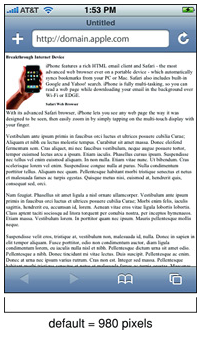
\includegraphics[scale=0.75]{viewport-default.png} \\
    Domyślnie w przeglądarce iOS Safari viewport wynosi 980 pikseli szerokości, mimo, iż ekran optymalnie wyświetla 320 pikseli. Aby przedstawić całą stronę internetową szerokość jest dobierana automatycznie.
\end{figure}

Podczas projektowania interfejsu strony internetowej wyświetlanej na stronie internetowej istotne jest okreslenie viewportu, aby uniknąć nieoczekiwanemu przyjęciu domyślnych wartości, bowiem strategie ich okreslania są różne. Niektóre przeglądarki dopasowują szerokość viewportu do najszerszego elementu strony internetowej, co powoduje, że tekst i elementy interaktywne mogą być niewidoczne. Aby przyjąć szerokość viewportu zgodne z szerokością przeglądarki internetowej na urządzeniu, należy zdefiniować wartość jako \lstinline{device-width}, wówczas szerokość strony zostanie przycięta, a w przypadku projektowania interfejsu zgodnie z zasadą Responsive Web Design (opisanum w podsekcji \ref{subsubsec:rwd}), istnieje możliwość określenia dedykowanych arkuszy styli definiujących wygląd strony w zależności od szerokości viewportu (który nie może być zmieniany na urządzeniu mobilnym, a w przypadku przeglądarki uruchomionej na komputerze - tak, poprzez zmianę rozmiaru okna).

\begin{figure}[h!]
  \caption[Apple fixed viewport w Safari iOS]{Ustawiony viewport iOS Safari na urządzeniu firmy Apple}
  \centering
    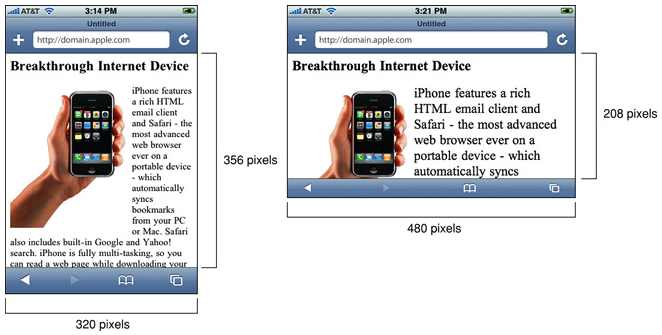
\includegraphics[scale=0.75]{viewport-adjusted.png} \\
    Viewport można regulować ustawiając stałe wartości, np 320px lub \lstinline{device-width} jako szerokość okna przeglądarki.
\end{figure}

\lstset{language=HTML}
\begin{lstlisting}
<meta name="viewport" content="width=device-width" />
\end{lstlisting}

\subsubsection{Cascading Style Sheet - Media Queries}

Znane są rozszerzenia kaskadowych arkuszy styli (ang. \emph{Cascading Style Sheet}, w skrócie \emph{CSS}) z wersji 2.1\cite{css21}, gdzie za pomocą atrybutu \emph{@media} istnieje możliwość zdefiniowania, jakiego typu urządzenia dotyczy wybrany arkusz styli\footnote{\cite{css21}, Rozdział \emph{Media types}}, tzw \emph{Media Queries}, np:

\begin{description}
  \item[all] \hfill \\
  Wszystkie urzadzenia
  \item[print] \hfill \\
  Dla urządzeń drukujących lub stron na ekranie wyświetlanych w trybie podglądu do wydruku.
  \item[handheld] \hfill \\
  Dla urządzeń kieszonkowych o zmniejszonej rozdzielczości ekranu.
  \item[projection] \hfill \\
  Dla urządzeń, które wyświetlają stronę w trybie prezentacyjnym, np projektorów.
  \item[tty] \hfill \\
  Dla urządzeń o ściśle określonym obszarze na wyświetlanie znaków, np. terminale, urządzenia przenośne z okraniczonym tekstowym wyświetlaczem.
  \item[all] \hfill \\
  c
\end{description}

Sposob załączania arkusza w zależności od jego przeznaczenia jest następujący dla dokumentu HTML:

\lstset{language=HTML}
\begin{lstlisting}
<link rel="stylesheet" type="text/css" href="layout.css"
  media="screen" />
<link rel="stylesheet" type="text/css" href="print.css"
  media="print" />
\end{lstlisting}

Lub bezpośrednio w arkuszu stylów:

\lstset{language=Octave}
\begin{lstlisting}
@media print {
  body { font-size: 10pt }
}
@media screen {
  body { font-size: 13px }
}
@media screen, print {
  body { line-height: 1.2 }
}
\end{lstlisting}

Nie jest to jednak wystarczające w kontekście dostosowania strony internetowej do rozmiarów i rozdzielczości okna przeglądarki. W CSS w wersji 3.1 wprowadzono możliwość załączania styli w zależności od rozdzielczości dostępnej powierzchni (\emph{viewport}) za pomocą rozszerzonego o tę możliwość \emph{Media Queries}\cite{css3}\footnote{\cite{css3} Rozdział \emph{Media Queries}, http://www.w3.org/TR/css3-mediaqueries/}.

Pojawiła się między innymi wartość atrybutu \lstinline{@media}: \lstinline{device-width} oraz \lstinline{device-height} z przedrostkami \lstinline{min-} i \lstinline{max-}, co w pełni wyczerpuje potrzeby projektowania stron internetowych zgodnie z RWD.

Przykładowy kod ładujący arkusz styli dla urządzeń o maksymalnej szerokości 480px:

\lstset{language=Octave}
\begin{lstlisting}
<link rel="stylesheet" type="text/css"
  media="screen and (max-device-width: 480px)"
  href="landscape.css" />
\end{lstlisting}
